\RequirePackage{lineno}
\documentclass[twocolumn,nofootinbib,showpacs,prl,superscriptaddress,secnumarabic,amssymb,nobibnotes,aps,floatfix]{revtex4}
\usepackage{graphicx}
\usepackage{hyperref}
\usepackage{amsmath}
\usepackage{dcolumn}% Align table columns on decimal point
\usepackage{bm}% bold math
%
\def\Dirac#1{#1\hskip-5pt/}
%
\newcommand*\patchAmsMathEnvironmentForLineno[1]{%
\expandafter\let\csname old#1\expandafter\endcsname\csname #1\endcsname
\expandafter\let\csname oldend#1\expandafter\endcsname\csname end#1\endcsname
\renewenvironment{#1}%
{\linenomath\csname old#1\endcsname}%
{\csname oldend#1\endcsname\endlinenomath}}%
\newcommand*\patchBothAmsMathEnvironmentsForLineno[1]{%
\patchAmsMathEnvironmentForLineno{#1}%
\patchAmsMathEnvironmentForLineno{#1*}}%
\AtBeginDocument{%
\patchBothAmsMathEnvironmentsForLineno{equation}%
\patchBothAmsMathEnvironmentsForLineno{align}%
\patchBothAmsMathEnvironmentsForLineno{flalign}%
\patchBothAmsMathEnvironmentsForLineno{alignat}%
\patchBothAmsMathEnvironmentsForLineno{gather}%
\patchBothAmsMathEnvironmentsForLineno{multline}%
}


%
\begin{document}
%\linenumbers

\title{Revealing the Bound Nucleon 3D Partonic Structure through Incoherent 
Deeply Virtual Compton Scattering off $^4$He}

\input author_list.tex

%
\date{\today}
\begin{abstract}
We report on the beam-spin asymmetries associated with incoherent deeply 
   virtual Compton scattering off $^4$He in the valence quark region.  The data 
   have been accumulated using a 6 GeV longitudinally-polarized electron beam 
   incident on a pressurized $^4$He gaseous target placed in front of the CLAS 
   spectrometer in Hall-B at Thomas Jefferson National Accelerator Facility.  
   The baseline detection sub-systems of CLAS detected the scattered electrons 
   and the recoil protons, while the final-state real photons are detected by a 
   supplementary electromagnetic calorimeter at very forward angles. The 
   measured beam-spin asymmetries on bound-protons exhibit a suppression 
   compared to those on free proton, indicating possible medium modifications 
   on the nucleon's quark distributions and opening new opportunities to 
   explore the origin of the EMC effect within the framework of the generalized 
   parton distributions.

\end{abstract}
\pacs{Valid PACS appear here}

\maketitle 

Electromagnetic probes have played a major role in advancing our knowledge 
about the structure of nucleons, which are the origin of almost all the
Universe visible matter. While the elastic lepton-nucleon measurements have 
taught us about the spatial charge and magnetization distributions 
\cite{Hofstadter:1955ae,Perdrisat:2006hj}, the deep-inelastic scattering (DIS) 
experiments have uncovered the features of momentum sharing between the 
constituents partons, i.e., quarks and gluons \cite{Dokshitzer:1977sg,pdg}. 
With nuclear targets, the DIS measurements have revealed the fact that the 
distribution of quarks in a fast moving nucleus is not a simple convolution of 
their distributions within nucleons, known as the ``EMC 
effect''\cite{EMC_first} (for reviews on the extensive investigations, see  
\cite{EMC_CERN,EMC_SLAC,EMC_HERMES,EMC_JLab,EMC_John,EMC_mdeium_1,EMC_medium_2}).

A wealth of information on the structure of matter lies in the correlations 
between the momentum and spatial degrees of freedom of the partons. These 
correlations are set to be revealed through deeply virtual Compton scattering 
(DVCS), i.e., the hard exclusive lepto-production of a real photon, which 
provide access to a three-dimensional imaging of partons within the generalized 
parton distributions (GPDs) framework 
\cite{Mueller:1998fv,Ji:1996ek,Ji:1996nm,Radyushkin:1996nd,Radyushkin:1997ki}.   
The free proton DVCS measurement has been the focus of a worldwide effort 
\cite{Stepanyan:2001sm,Airapetian,Chekanov:2003ya,Aktas:2005ty,Chen:2006na,Munoz 
Camacho:2006hx,Girod:2007aa,Mazouz:2007aa,Gavalian:2009,Seder:2015,Pisano:2015,Jo:2015ema}
involving several accelerator facilities such as Jefferson Lab (JLab), HERA and  
CERN. Combining these measurements has enabled the first tomography extraction 
of the free proton \cite{Dupre:2016mai}. New groundbreaking measurements of 
exclusive DVCS from the $^{4}$He nucleus are a critical step towards providing 
similar 3D pictures of the quark structure of the nucleus as a whole, via the 
coherent channel \cite{Hattawy:2017woc}, and provide a new approach to 
understanding the partonic modifications of the bound nucleons via the 
incoherent DVCS channel \cite{simonetta_2,Guzey:2006xi,Guzey:2008fe}. The 
$^{4}$He nucleus is an ideal experimental target for these purposes as it has 
only one chiral-even GPD that parametrizes its partonic structure, is 
characterized by a strong binding energy, and has a relatively high nuclear 
core density. The inclusive scattering off $^{4}$He has shown a large EMC 
effect \cite{JSeely}, making this nucleus a golden target for investigating the 
medium partonic modifications. 


\begin{figure}[tb]
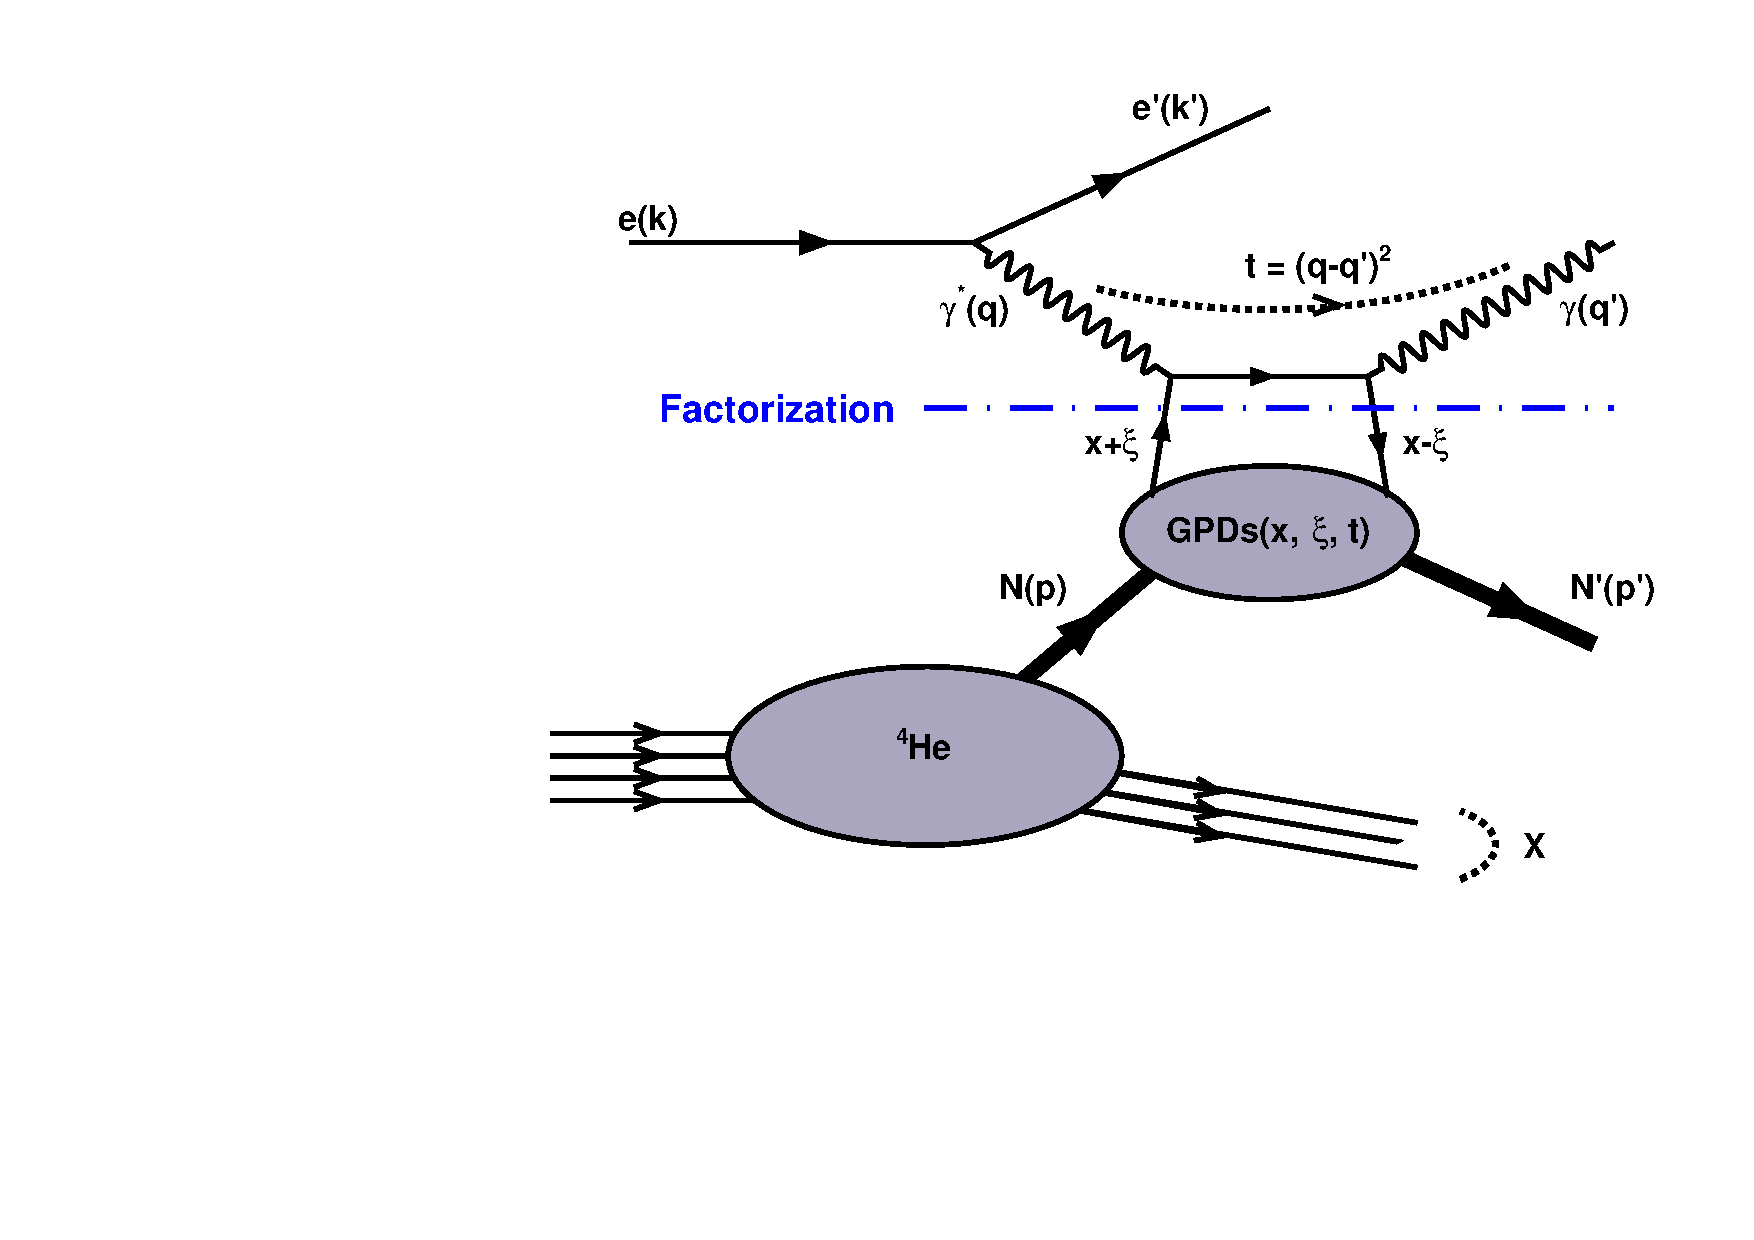
\includegraphics[width=7.5cm]{figs/handbag_incoherent.pdf}
\caption{Representation of the leading-order, twist-2, handbag diagram of the 
   incoherent DVCS process off $^4$He, where the four-vectors of the electrons, 
   photons, and protons are denoted by $k/k^\prime$, $q/q^\prime$, and 
   $p/p^\prime$, respectively. $x+\xi$ is the nucleon’s longitudinal momentum 
   fraction carried by the struck quark, 2$\xi$ is the longitudinal momentum 
   fraction of the momentum transfer $\Delta$ ($= p - p^\prime$), and 
   $t$~($=\Delta^2$) is the squared momentum transfer between the initial and
   the final state nucleon.}
\label{fig:diags}
\end{figure}

FIG.~\ref{fig:diags} illustrates a schematic representation of the 
leading-twist handbag diagram for the incoherent DVCS off $^{4}$He. In the 
Bjorken region, i.e, large virtual photon four-momentum squared 
($Q^{2}=-(k-k^\prime)^2$), and at small invariant momentum transfer ($t$), the 
DVCS handbag diagram can be factorized, leaving the non-perturbative structure 
of the nucleon to be parametrized in terms of four chirally-even GPDs: $H$, 
$E$, $\widetilde{H}$, and $\widetilde{E}$, representing the four helicity-spin 
combinations of the quark-nucleon states \cite{Freund_Collins,Ji_Osborne}.

In this Letter, we present the beam-spin asymmetries associated with the photon 
electroproduction on bound-proton off $^{4}$He. While the experimentally 
measured cross section amplitude is the sum of the DVCS, BH (i.e., the final 
state real photon is emitted by the incident or the scattered electron), and 
their interference, the beam-spin asymmetry observable is sensitive to the 
amplitudes that contain information on the GPDs, i.e., DVCS and interference 
amplitudes. The beam-spin asymmetry observable is measurable using a polarized 
lepton beam on unpolarized target (U) and defined in terms of the cross 
sections as
\begin{equation}
  A_{LU} = \frac{d^{5}\sigma^{+} - d^{5}\sigma^{-} }
                {d^{5}\sigma^{+} + d^{5}\sigma^{-}}.
    \label{BSA_equation}
  \end{equation}
where $d^{5}\sigma^{+}$($d^{5}\sigma^{-}$) is the photon electroproduction 
differential cross section for a positive (negative) beam helicity. 

Following the cross section decomposition suggested by \cite{Belitsky:2001ns}, 
the different amplitudes can be expressed in terms of Fourier coefficients 
associated with $\phi$-harmonics, where $\phi$ is the angle between the 
leptonic and the hadronic planes of the reaction. At leading-twist, the 
beam-spin asymmetry can be simplified as \begin{equation}
   A_{LU}(\phi) = \frac{a_{0}\sin(\phi)}{1+a_{1}\cos(\phi)+a_{2}\cos(2\phi)}
   \label{eq:alu-simp}
\end{equation}
with the parameters $a_{0,1,2}$ are combinations of the above mentioned Fourier 
coefficients. The first sine harmonic of the beam-spin asymmetry is dominant 
and proportional to the following combination of Compton form factors (CFF) 
\cite{Guidal:2013rya}
\begin{equation}
   A_{LU}^{\sin\phi} \propto \operatorname{Im}( F_1 \mathcal{H}- \frac{t}{4M^2} 
   F_2 \mathcal{E}+ \frac{x_B}{2}(F_1+F_2)\tilde{\mathcal{H}})
\end{equation}
where $F_1$ and $F_2$ are the Dirac and Pauli form factors with $x_B$ as the 
Bjorken scaling variable. The real and the imaginary parts of the CFF 
$\mathcal{H}$ are corresponding to the GPD $H$ by  \begin{align}
   \Re(&\mathcal{H}) = \mathcal{P} \int_{0}^{1}dx[H(x,\xi,t)-H(-x,\xi,t)] \, 
   C^{+}(x,\xi) \\
   \Im(&\mathcal{H}) = - \pi [H(\xi,\xi,t)-H(-\xi,\xi,t)],
\end{align}
with $\mathcal{P}$ is the Cauchy principal value integral and $C^{+}$ is a 
coefficient function defined as $(1/(x-\xi) + 1/(x+\xi))$ with $\xi$ being 
related to $x_B$ by $\xi\approx {{x_B}\over{2-x_B}}$. Similar expressions apply 
for the GPDs $E$, $\widetilde{H}$, and $\widetilde{E}$.

%experimental setup

The experiment (E08-024~\cite{Hafidi:2008pr}) took place in Hall-B of Jefferson 
Lab using the nearly 100\% duty factor, longitudinally-polarized electron beam 
(83$\%$ polarization) from the Continuous Electron Beam Accelerator Facility 
(CEBAF) accelerator at its full energy of 6.064 GeV. The data were accumulated 
over 40 days using a 6-atm-pressure, 292-mm-long, and 6-mm-diameter gaseous 
$^4$He target centered at 64~cm upstream of the CEBAF Large Acceptance 
Spectrometer (CLAS) center. For similar DVCS experiments on free-proton target
\cite{Girod:2007aa,Jo:2015ema}, the CLAS baseline design \cite{Mecking:2003zu} 
is supplemented with an inner calorimeter (IC) and a solenoid. The IC extends 
the photon detection acceptance of CLAS, which was originally from 15$^{\circ}$ 
to 45$^{\circ}$, to polar angles as low as 4$^{\circ}$. As the coherent DVCS 
off $^4$He, where the nucleus remain intact, was one of the proposed 
measurements of our experiment and since CLAS cannot detect such low-energy 
recoil nuclei, we built a small radial time projection chamber (RTPC) around 
the target cell. (See~\cite{Dupre:2017upj} for a detailed description of the 
RTPC and its performances and \cite{Hattawy:2017woc} for the coherent DVCS 
measurements). In this setup, the 5-Tesla solenoid (that surrounds the target 
and the RTPC) enabled the detection of the low-energy charged ions in the RTPC 
and prevented the high-rate low-energy M\o{}ller electrons from reaching CLAS 
sub-detectors by guiding these electrons towards a heavy shield placed around 
the beam line. 


% DVCS selection
Incoherent DVCS events were selected if an electron, a proton, and at least one 
photon were detected in the final state. Electrons were identified by having 
appropriate deposited energy in the electromagnetic calorimeter and proper 
light yield in the Cherenkov counters in addition to having a negative 
track-curvature in the drift chambers that corresponds to a momentum greater 
than 800 MeV. The protons were distinguished from other positive particles by 
timing cuts established using the time-of-flight measured by the scintillators 
and the reconstructed track information from the drift chambers. Also, the 
selected proton was required to be originating from the electron's vertex by 
applying a vertex matching cut. The photons were detected in either the IC or 
the CLAS electromagnetic calorimeter. All the signals within IC fiducial region 
were assumed to be photons, while a timing cut is used to clean the EC photons 
from neutrons. Note that even though the DVCS reaction has only one real photon 
in the final state, events with more than one good photon are not discarded at 
this stage. It was observed by the DVCS exclusivity cuts, discussed below, that 
most of these photons are soft ones produced in random coincidence. In the 
following selection stage, the most energetic photon is considered as the DVCS 
photon candidate (see \cite{Hattawy:thesis} for additional details on the 
particles identification).  

Further requirements were applied to clean the identified initial set of 
incoherent DVCS events from backgrounds and other channels. Events were 
selected with $Q^{2}$ greater the 1 GeV$^2$ to ensure that the interaction 
occurs at the partonic level and the applicability of the factorization on the 
DVCS handbag diagram, $\gamma^{*}p$ invariant mass (W) greater than 2 GeV to 
avoid the nucleon region of excitation to resonances, and the transferred 
momentum squared to the recoil proton has to be greater than a
minimum value defined by the kinematics of the beam and the scattered electron 
($-t~>~-t_{min}$). Then, the exclusivity of the incoherent DVCS events was 
ensured by imposing constraints on the kinematical variables resulting from 
conserving the four-momentum in the reaction $ep\rightarrow e'p'\gamma$. These 
kinematical variables are: the coplanarity angle $\Delta\phi$ between the 
($\gamma,\gamma^*$) and ($\gamma^*$,$p'$) planes, the missing energy, mass, and 
transverse momentum of the $e'\gamma$ and $e'p'\gamma$ system, the missing mass 
squared of the $e'p'$ system, and the angle $\theta$ between the measured 
photon and the missing momentum of the $e'p'$ system. The experimental data for 
the most relevant exclusivity variables and applied cuts are shown in 
FIG.~\ref{fig:kin-cuts} (see \cite{Hattawy:thesis} for additional details). We 
also rejected events where a $\pi^0$ was identified by the invariant mass of 
two photons. About 30k events passed all these requirements; their kinematic 
distributions are shown in FIG.~\ref{fig:kin-coverage}.  

\begin{figure}[tb]
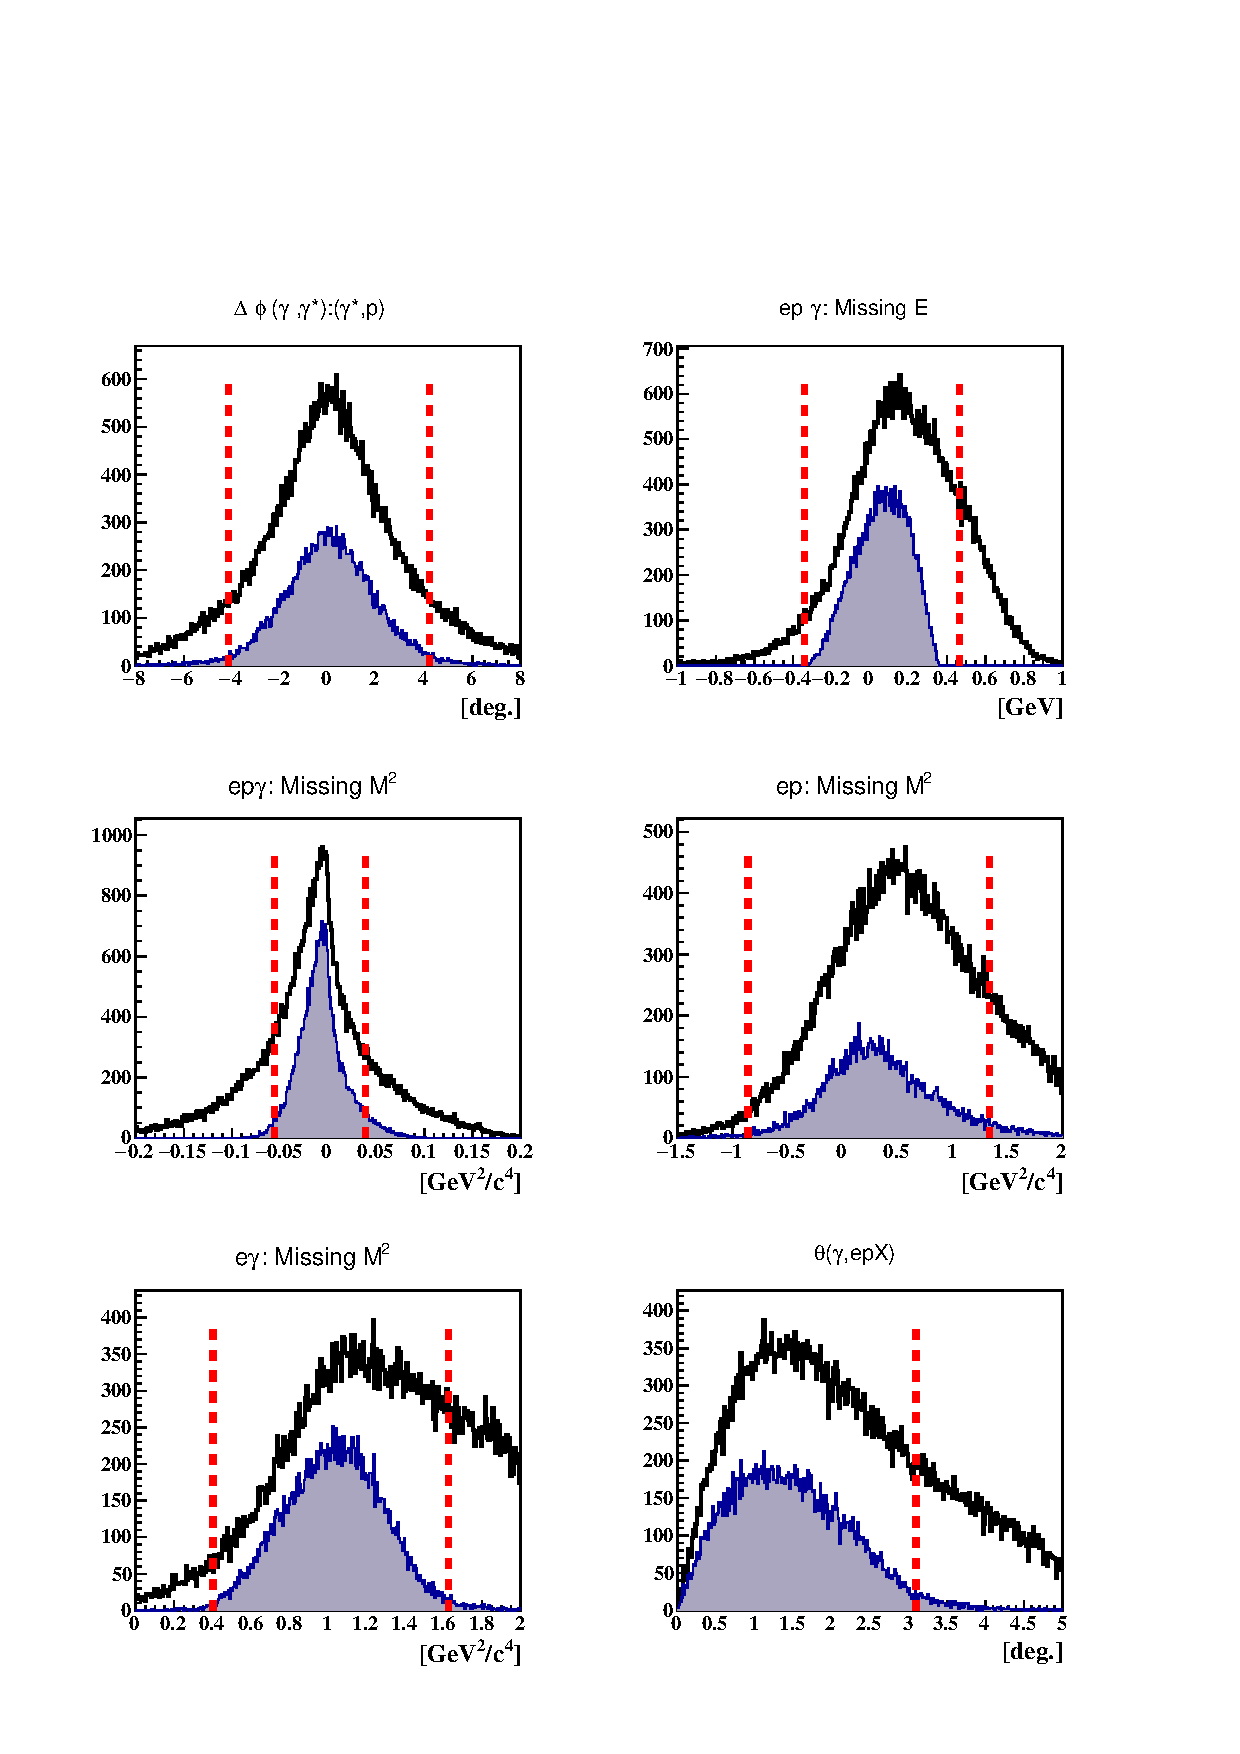
\includegraphics[width=8.9cm]{figs/incoh_exc_cuts_final.pdf}
\caption{The incoherent DVCS exclusivity cuts. The black distributions 
   represent the incoherent DVCS events candidate before all the exclusive 
   cuts. The shaded distributions represent the incoherent DVCS events which 
   passed all the exclusivity cuts except the quantity plotted. The vertical 
   red lines represent the applied exclusivity cuts. The distributions from 
   left to right and from top to bottoms are: $\Delta \phi$, missing energy,
   missing masses squared and the cone angle ($\theta$) between the measured 
   and the calculated photons in the $e'p'$ final-state system. }
\label{fig:kin-cuts}

\end{figure}
\begin{figure}[h!]
\hspace{-0.45cm}
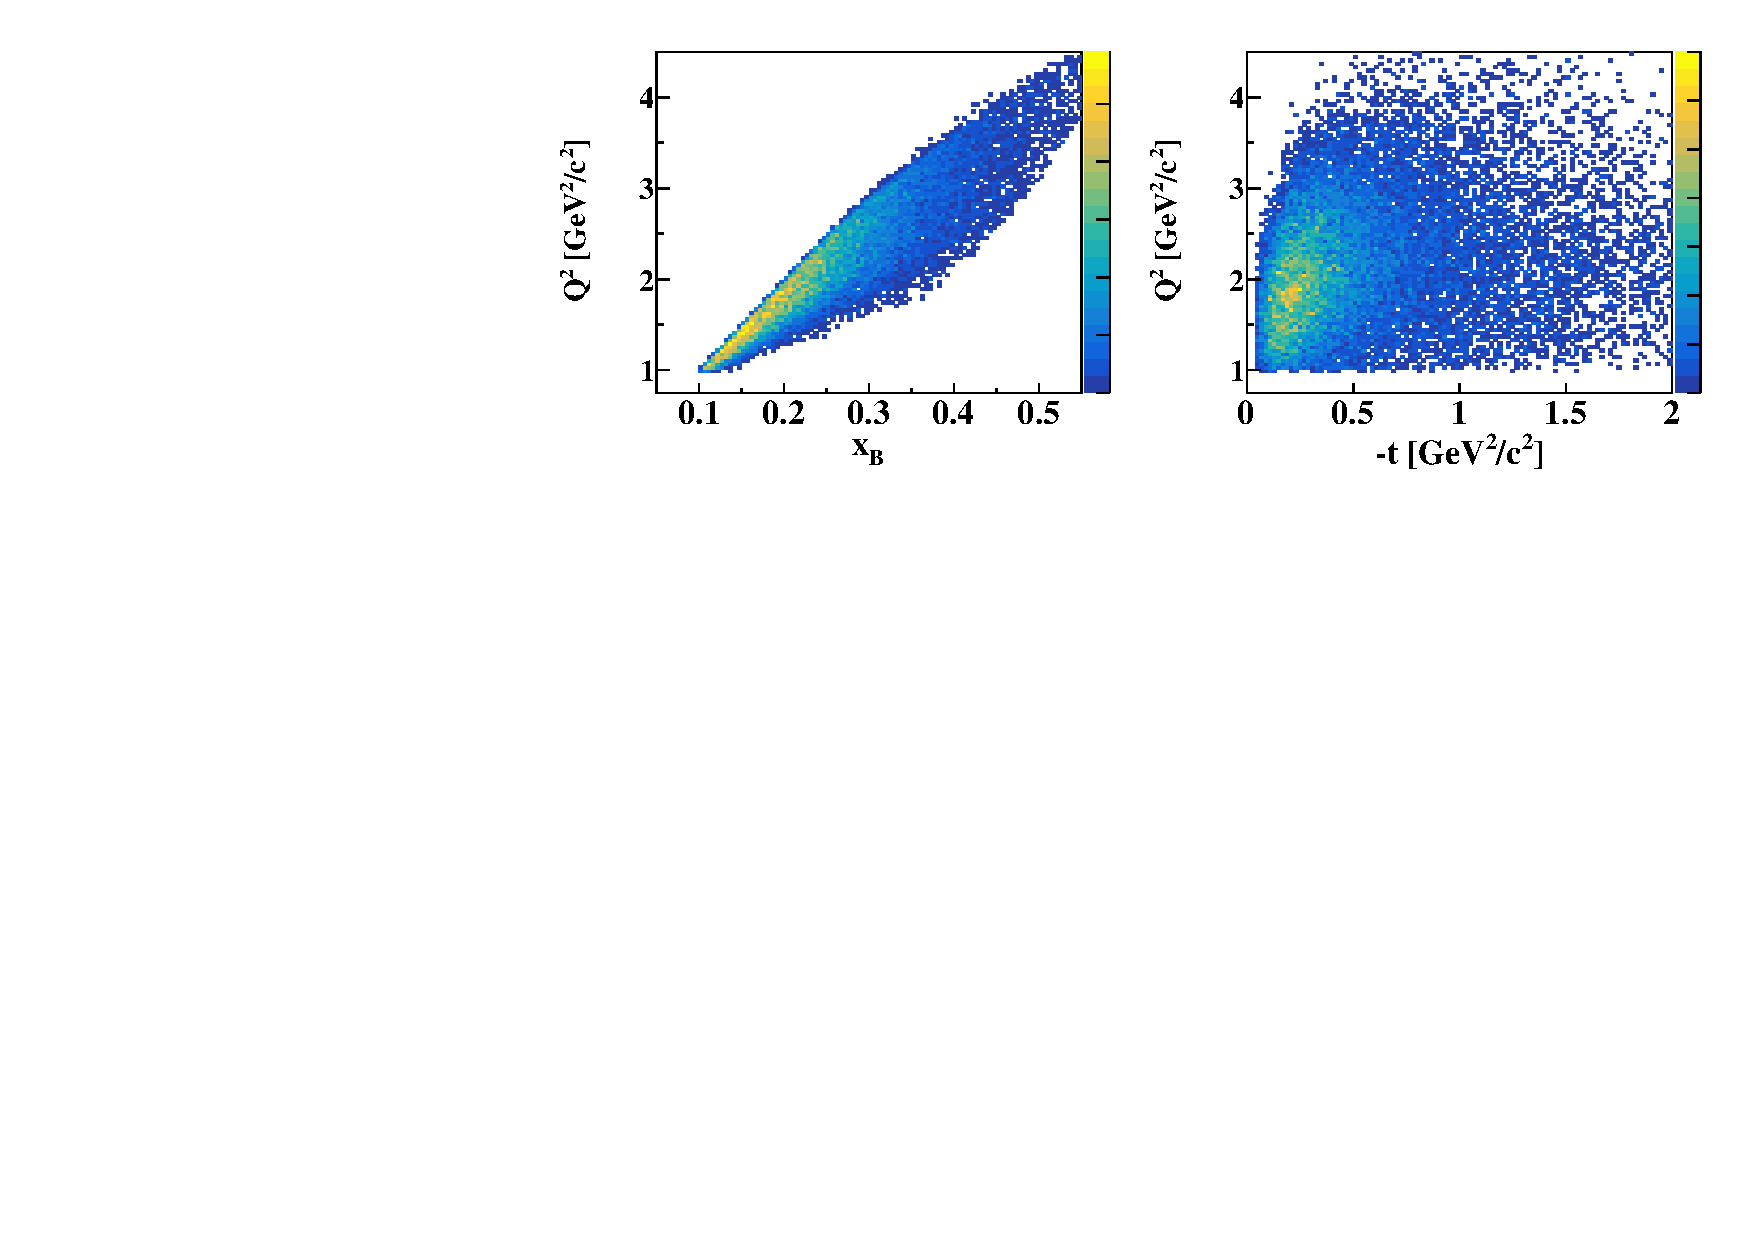
\includegraphics[width=9.0cm]{figs/Q2_xB_t_InCoh.pdf}
\caption{Incoherent DVCS event distributions for $Q^{2}$ as a function of 
$x_{B}$ (left) and $Q^{2}$ as a function of $-t$ (right) after the exclusivity 
cuts.}
\label{fig:kin-coverage}
\end{figure}


%background
In spite of our selection requirements, two main backgrounds were observed to 
contaminate our incoherent DVCS sample; accidental coincidences and exclusive 
$\pi^0$ production. For the accidental events, i.e., $e'p'\gamma$ collection 
with particles originated from different events, their contribution of 6.5\% 
was evaluated by selecting events passing all our cuts but originating from 
different vertices. Regarding the $\pi^0$ contamination, i.e., $ep\rightarrow 
e'p'\pi^0$ events where one of the two photons of the $\pi^0$ decay is produced 
below the energy threshold or outside the detection acceptance, we evaluated 
this contribution by using data and simulation. From the simulation, we 
calculated the ratio ($R$) between the number of $\pi^0$ events where the two 
photons are detected and those that would be mistaken for DVCS ($R = 
N^{1\gamma}_{sim}/N^{2\gamma}_{sim}$). Then in each kinematical bin and for 
each beam-helicity state, the $\pi^0$-subtracted experimental DVCS events is 
calculated as $N = N^{ep\rightarrow e'p'\gamma}_{exp}- R~N^{ep\rightarrow 
e'p'\pi^0}_{exp}$, where $N^{ep\rightarrow e'p'\gamma}_{exp}$ is the 
experimentally identified number of $ep\rightarrow e'p'\gamma$ and 
$N^{ep\rightarrow e'p'\pi^0}_{exp}$ is the experimentally identified 
$ep\rightarrow e'p'\pi^0$ with the two photons were detected. Depending on the 
kinematics, we found contaminations of 8\%-10\%. 



%asymmetries
It is convenient to use the beam-spin asymmetry as a DVCS observable because  
the cross sections luminosity normalization and detector efficiencies cancel 
out in the asymmetry ratio.  Experimentally, $A_{LU}$ can be simplified in 
terms of the reaction yield in each beam-helicity state ($N^{\pm}$) as
\begin{equation}
A_{LU} = \frac{1}{P_{B}} \frac{N^{+} - N^{-}}{N^{+} + N^{-} }.
\end{equation}
where $P_{B}$ is the longitudinal beam polarization.  

Following the model guidance of \cite{Guidal:2013rya}, the GPD $H$ dominants 
the other three GPDs within the accessible phase-phase of using the 6 GeV 
electron beam from CEBAF and CLAS spectrometer. Therefore, measuring $A_{LU}$ 
gives access to the real and imaginary part of the CFF $\mathcal{H}$ through 
the parameters $a_0$, $a_1$, and $a_2$ of equation \ref{eq:alu-simp}.  
Moreover, the free proton $A_{LU}$ measurements, \cite{Girod:2007aa}, have 
shown that the $cos(2\phi)$ term, which is corresponding to the pure DVCS 
amplitude, is suppressed and compatible with zero.  

Due to limited statistics, the data were binned two-dimensionally into 36 bins.  
That is, four statistically-equivalent bins in each of the kinematical 
variables ($Q^{2}$, $x_{B}$, $t$) were constructed one at a time. Then, each 
bin is divided into nine bins in the azimuthal angle ($\phi$).  
FIG.~\ref{fig:alu} presents the measured incoherent $A_{LU}$ as a function of 
$\phi$ in bins in $Q^{2}$, $x_{B}$, and $t$. The curves on the plots are fits 
of the approximated form $\frac{a_{0}~sin(\phi)}{1+ a_{1}~cos(\phi)}$. The 
study of systematic uncertainties showed that the main contributions come from 
the choice of the DVCS exclusivity cuts (6\%) and the large binning size (7\%).  
However, added quadratically, these uncertainties sum up to about 10\%, which 
always remains significantly smaller than the statistical errors.

\begin{figure}[tb]
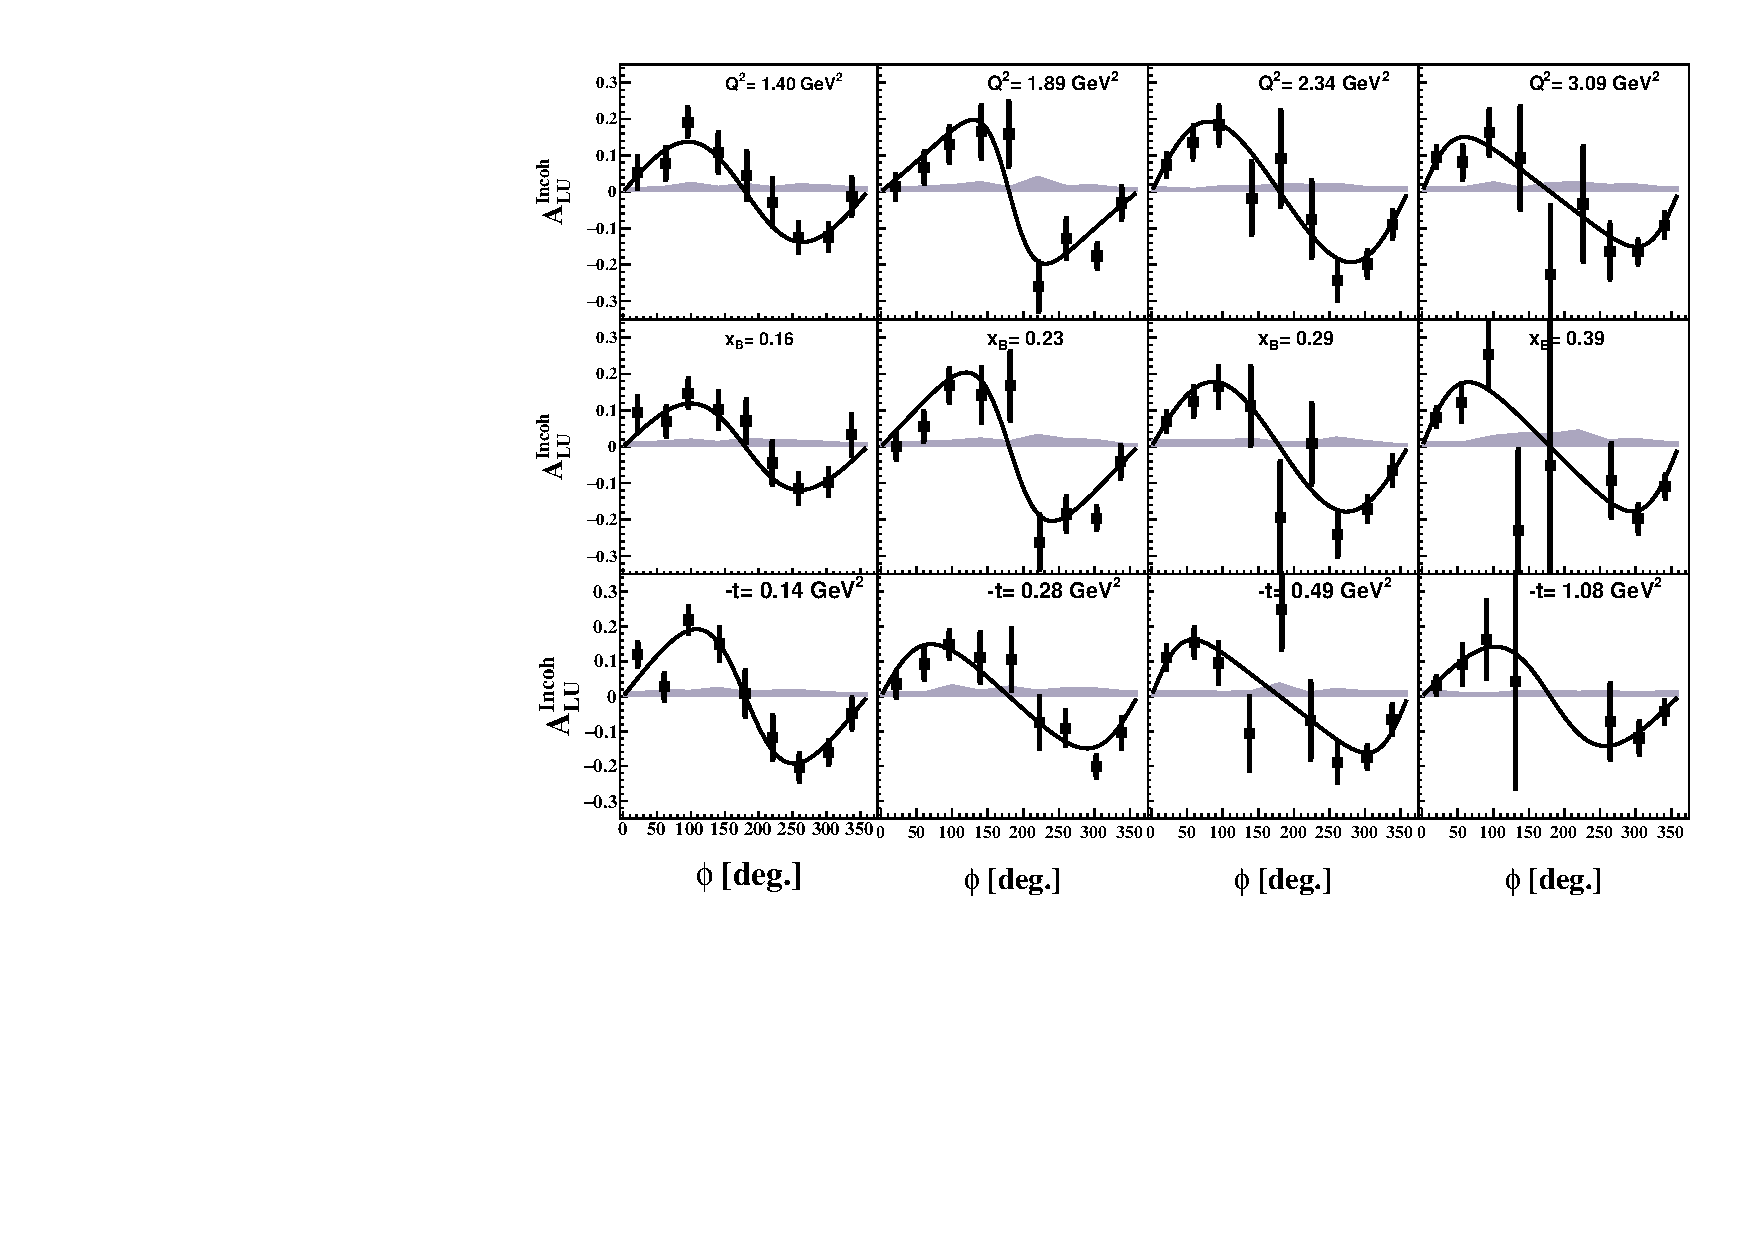
\includegraphics[width=8.9cm]{figs/incoherent_ALU_phi.pdf}
\caption{The incoherent $A_{LU}$ as a function of $\phi$. Results are presented
   for different $Q^{2}$ bins (top panel), $x_{B}$ bins (middle panel), and 
   $-t$ bins (bottom panel). The error bars represent the statistical 
   uncertainties. The gray bands represent the systematic uncertainties, 
   including the normalisation uncertainties. The black curves are the results 
   of our fits with the form $\frac{a_{0}~sin(\phi)}{1+ a_{1}~cos(\phi)}$.}
\label{fig:alu}
\end{figure}


We present in FIG.~\ref{fig:alu90} the dependence of the fitted $A_{LU}$ 
signals at $\phi$~=~90$^{\circ}$ on the kinematical variables $Q^2$, $x_{B}$, 
and $t$. Within the given uncertainties, $A_{LU}$ does not indicate a strong 
dependence on $Q^2$. The $x_{B}$ and $t$ dependencies are compared to 
theoretical calculations performed by S.~Liuti and K.~Taneja 
\cite{simonetta_2}. Their model uses a realistic spectral function and 
considers off-shell effects. The calculations are carried out at slightly 
different kinematics than our data but still provide some guidance. The 
experimental results appear to have smaller asymmetries than the calculations.  
These differences may arise from nuclear effects which are not taken into 
account in the model, such as long-range interactions.

\begin{figure}[tb]
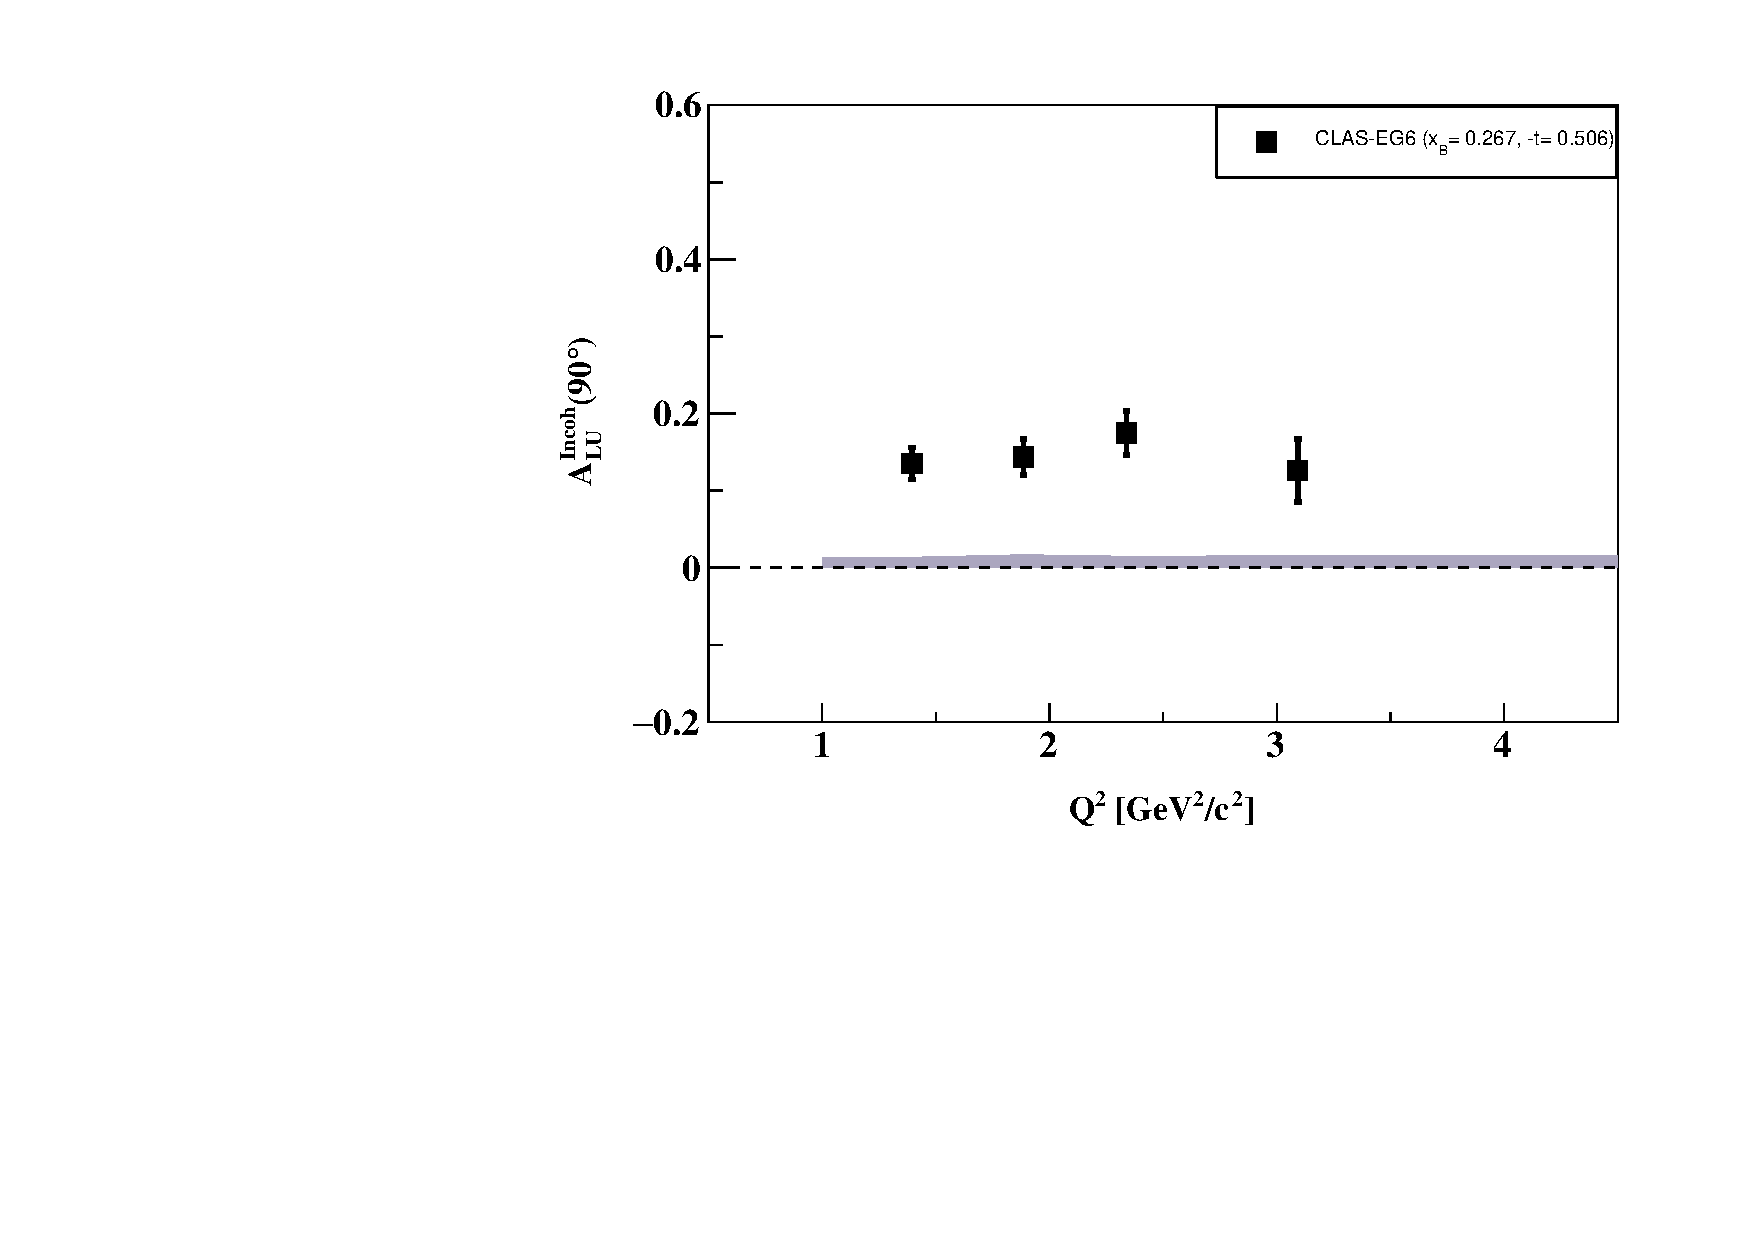
\includegraphics[width=6.9cm]{figs/ALU_90_p_vs_Q2_shortscenrario.pdf}
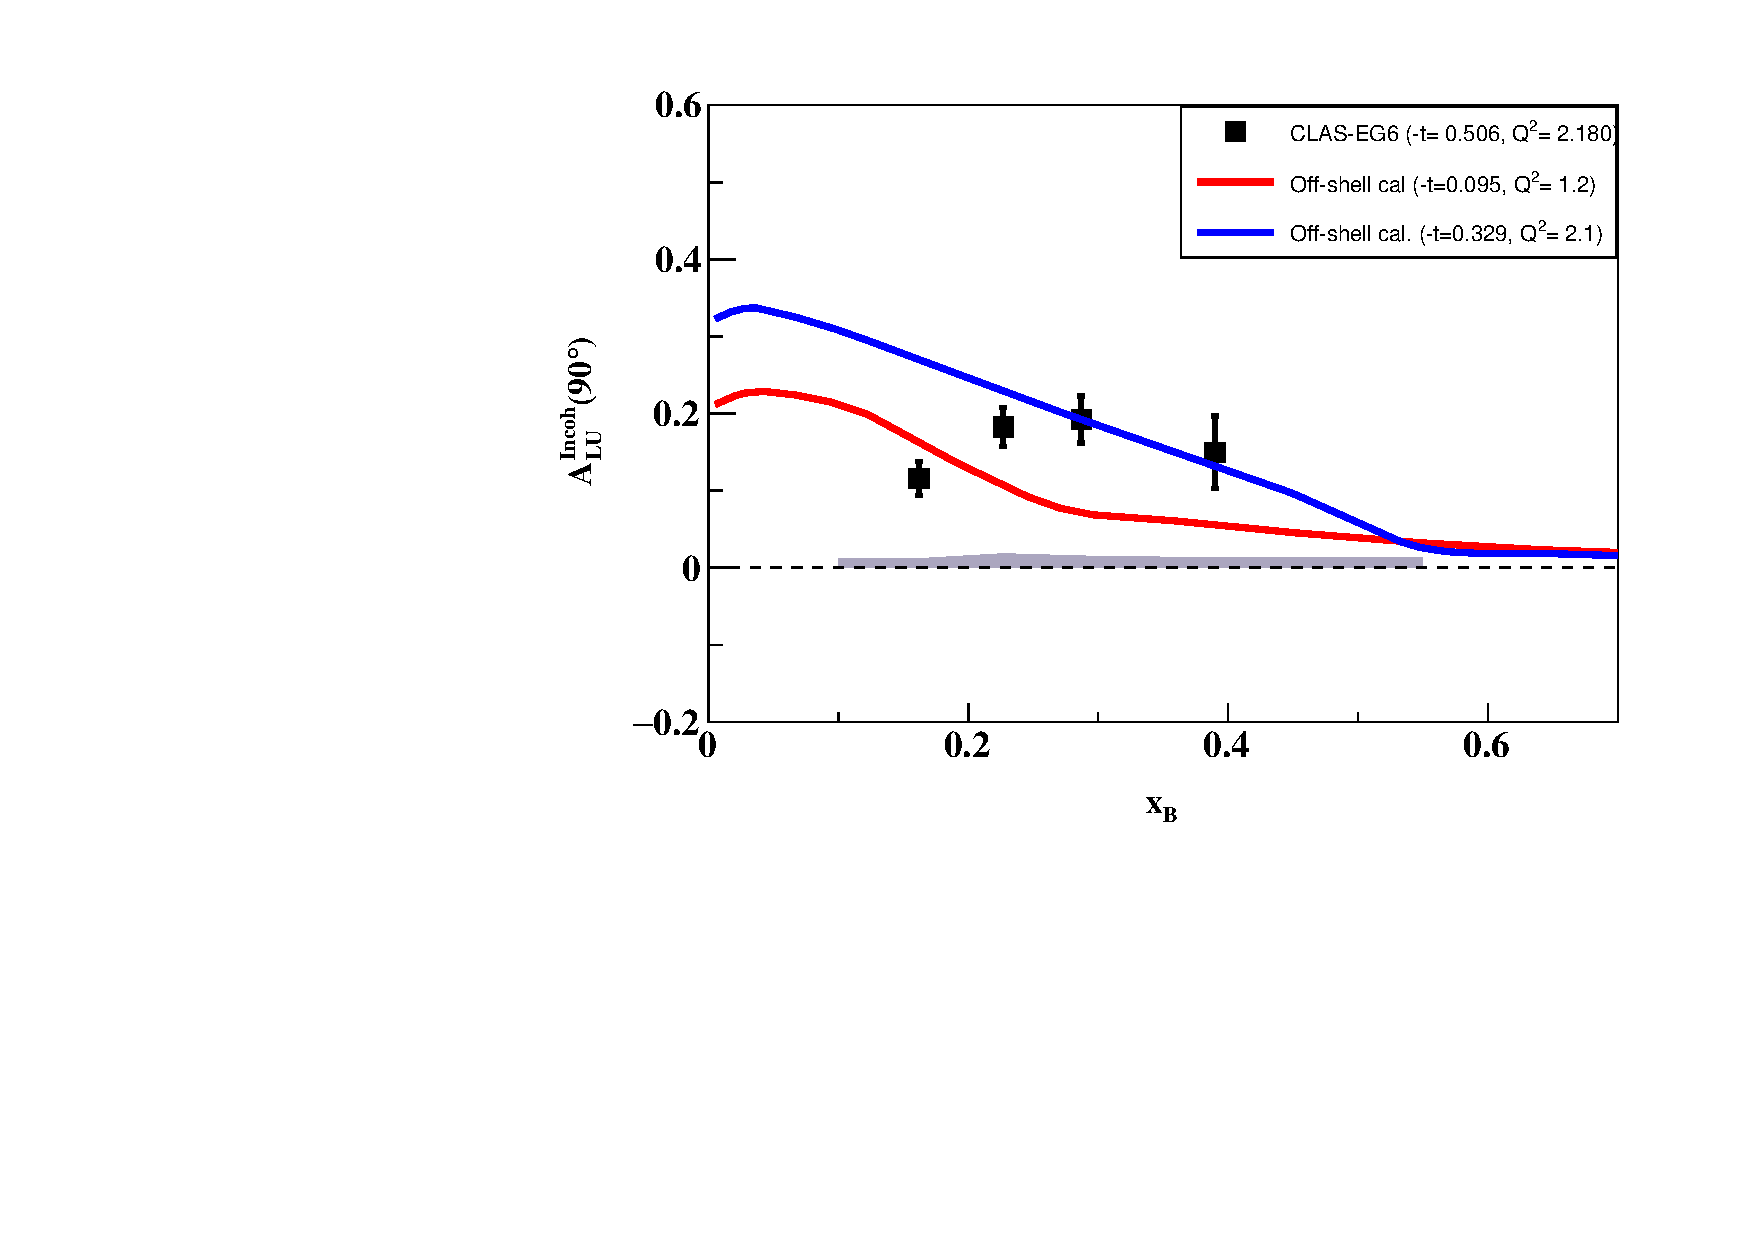
\includegraphics[width=6.9cm]{figs/ALU_90_p_vs_x_shortscenrario.pdf}
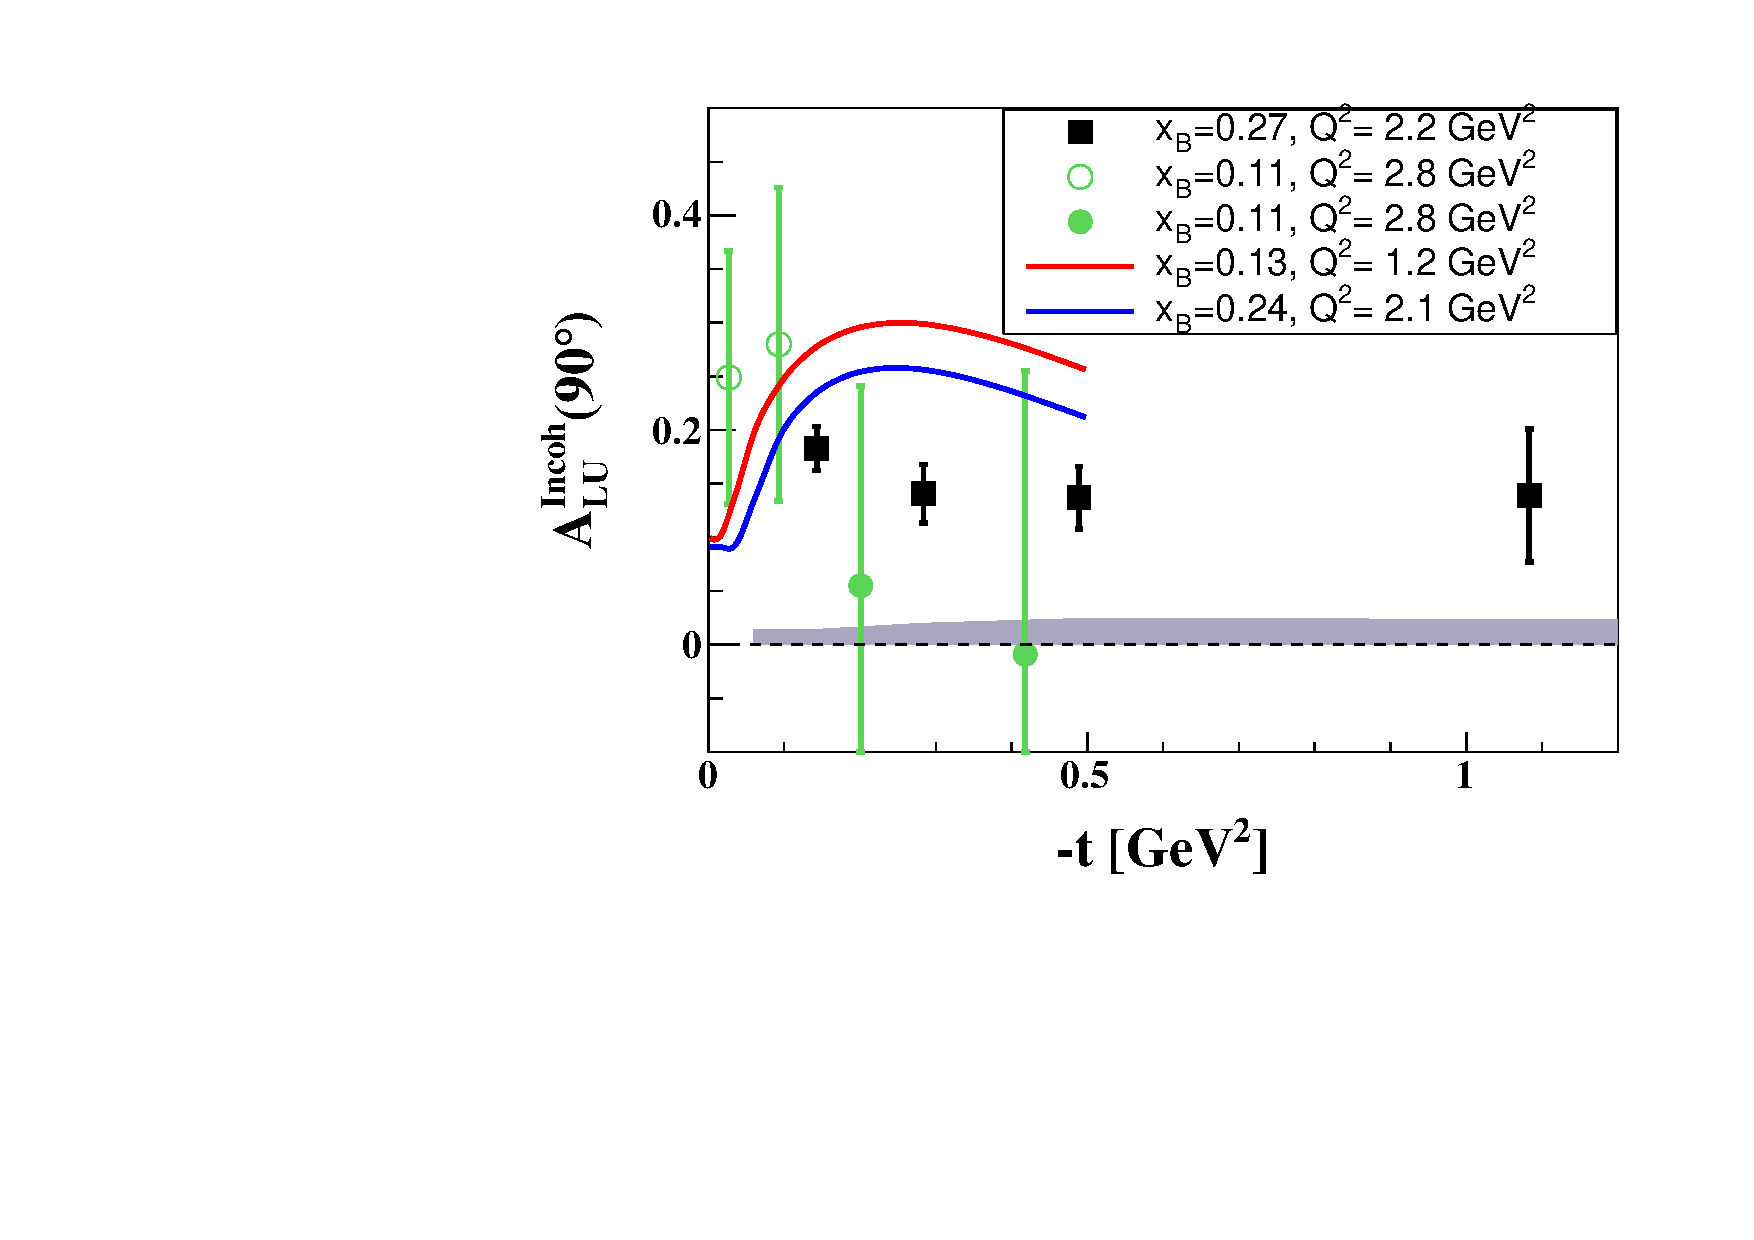
\includegraphics[width=6.9cm]{figs/ALU_90_p_vs_t_shortscenrario.pdf}
\caption{The $Q^{2}$ (top), $x_{B}$ (middle), and $t$ dependencies (bottom) of
   the fitted $A_{LU}$ at $\phi$~=~90$^{\circ}$ (black squares). The error bars 
   represent the statistical uncertainties, while the gray bands represent the 
   systematic uncertainties. On the middle plot: the curves are theoretical 
   calculations from \cite{simonetta_2}. On the bottom: the green circles are 
   the HERMES $-A_{LU}$ (positron beam was used) inclusive measurements 
   \cite{Airapetian}, the curves represent theoretical calculations from 
   \cite{simonetta_2}. } \label{fig:alu90}
\end{figure}

In this work we carried out the first step towards measuring the 
``generalized'' EMC effect in order to understand the potential sources of 
nuclear effects at the partonic level within the GPDs framework. We construct 
the ratio of $A_{LU}$ for bound protons to that on free proton target measured 
using similar electron-beam energy and experimental setup.  
FIG.~\ref{fig:incoh_EMC_ratio_ALU_proton} presents the dependence of the 
beam-spin asymmetry ratio at $\phi$~=~90$^{\circ}$ on the kinematical variables 
$Q^2$, $x_B$, and $t$. The free proton asymmetries were interpolated from the 
published results \cite{Girod:2007aa}.   

\begin{figure}[tb]
\centering
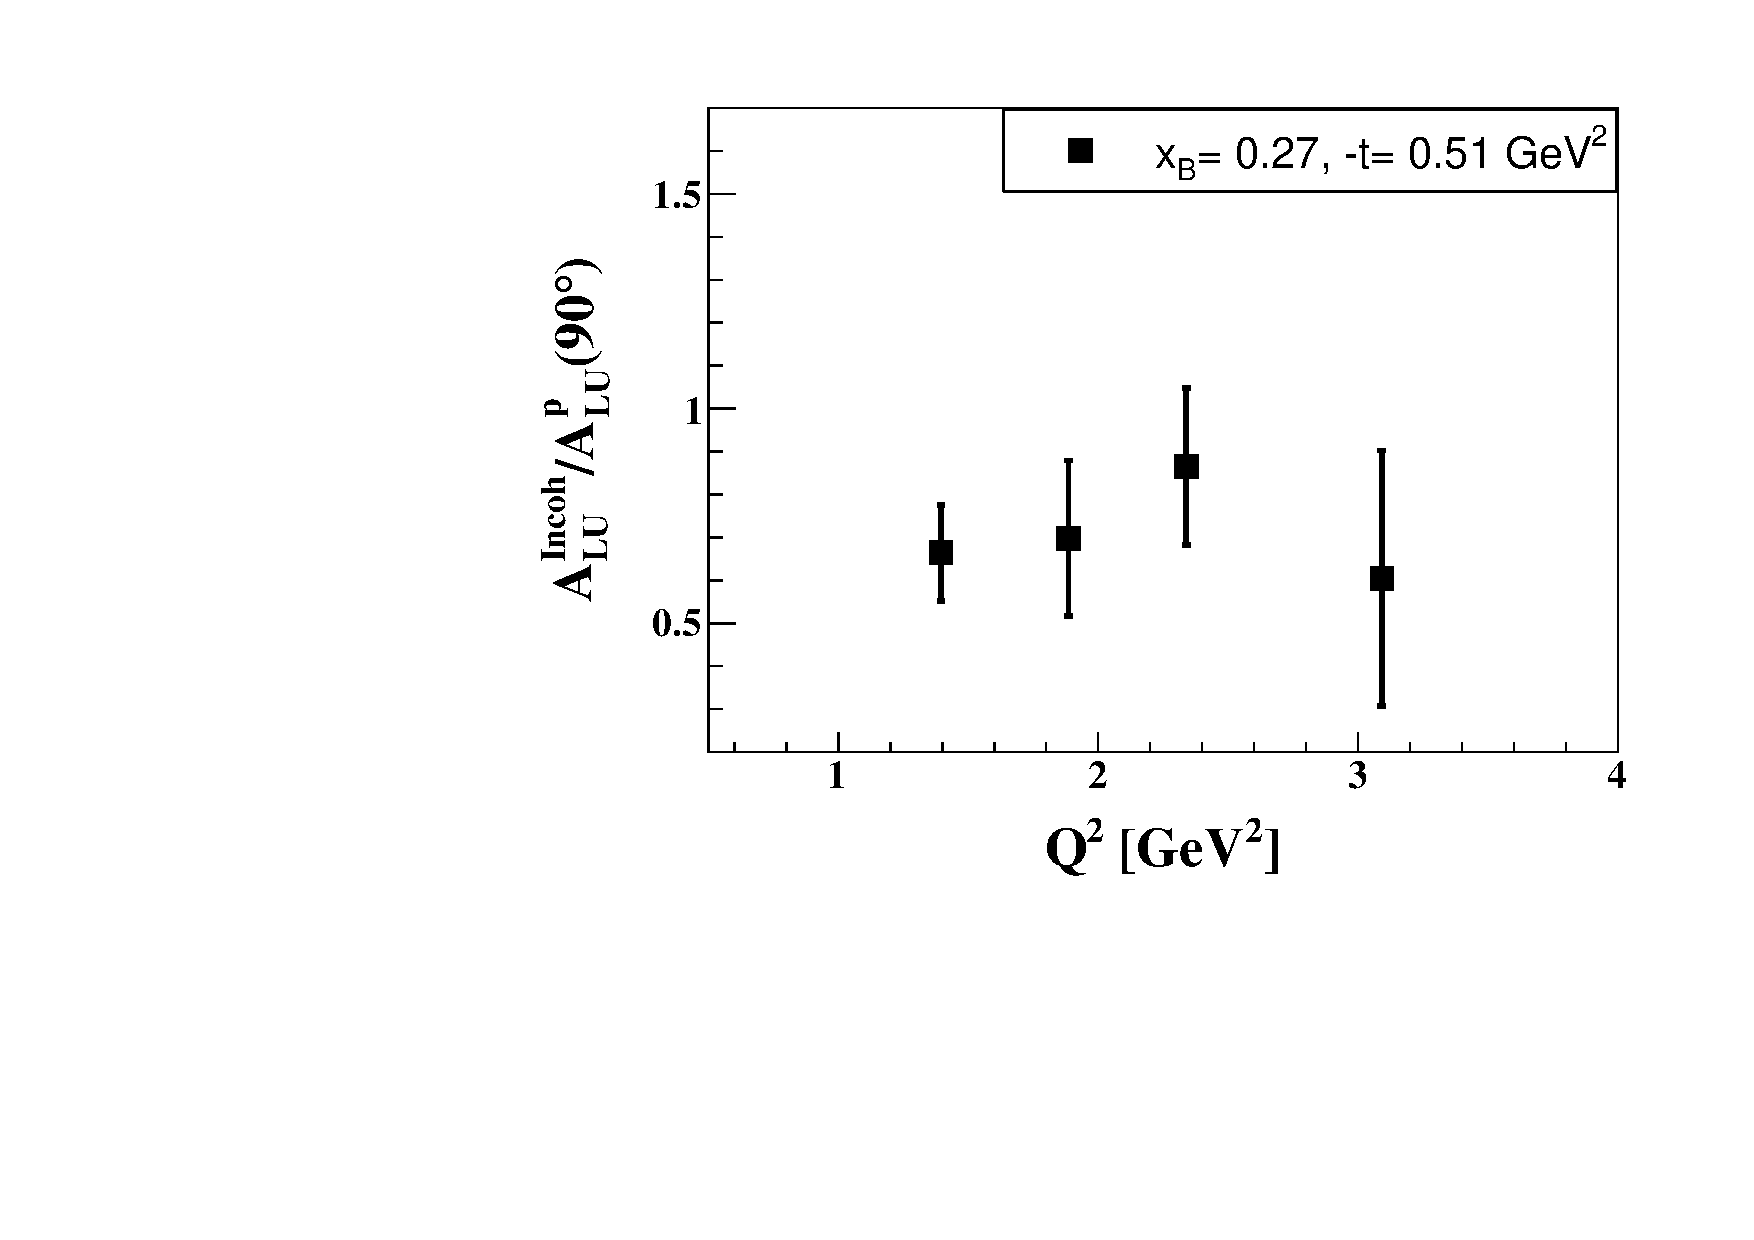
\includegraphics[width=6.9cm]{figs/ALU_ratioInc_Q2_shortscenrario.pdf}\\
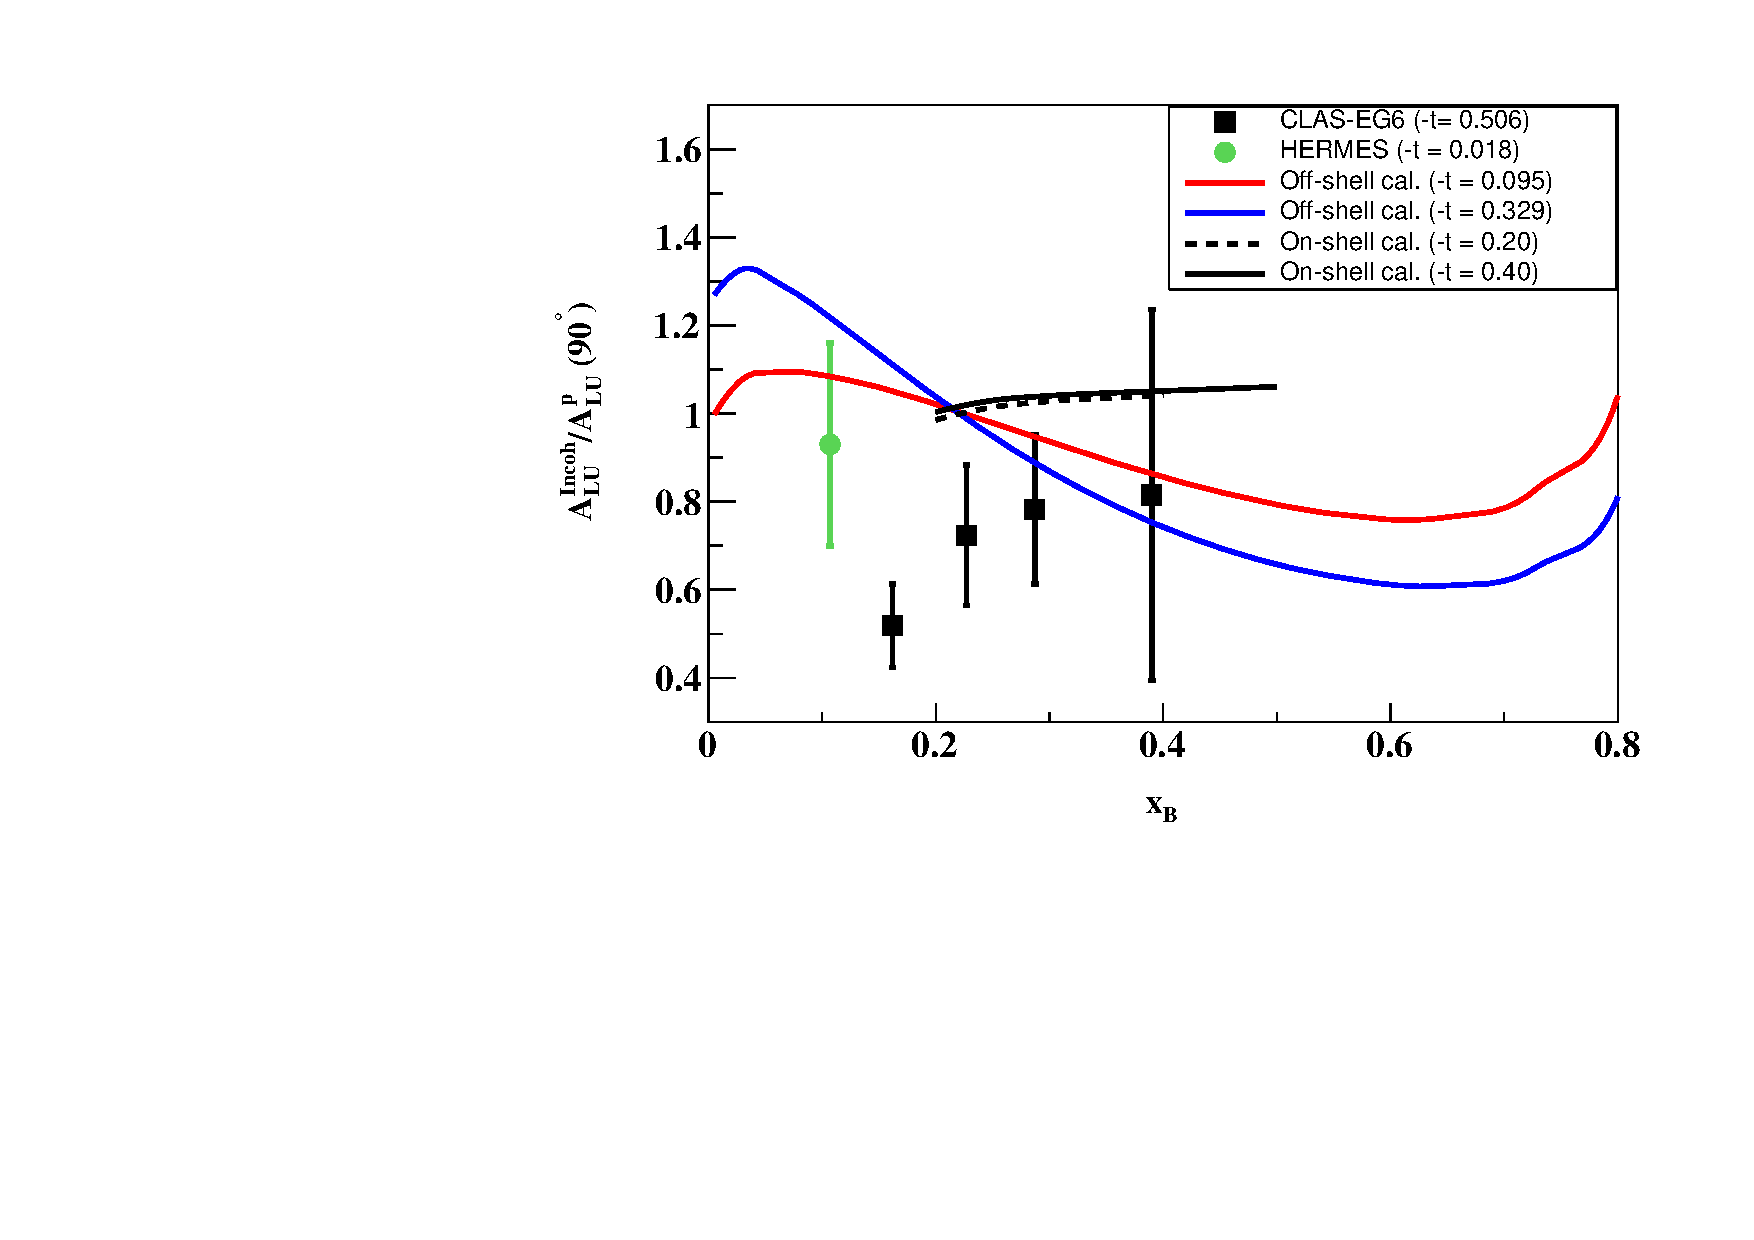
\includegraphics[width=6.9cm]{figs/ALU_ratioInc_x_shortscenrario.pdf}\\
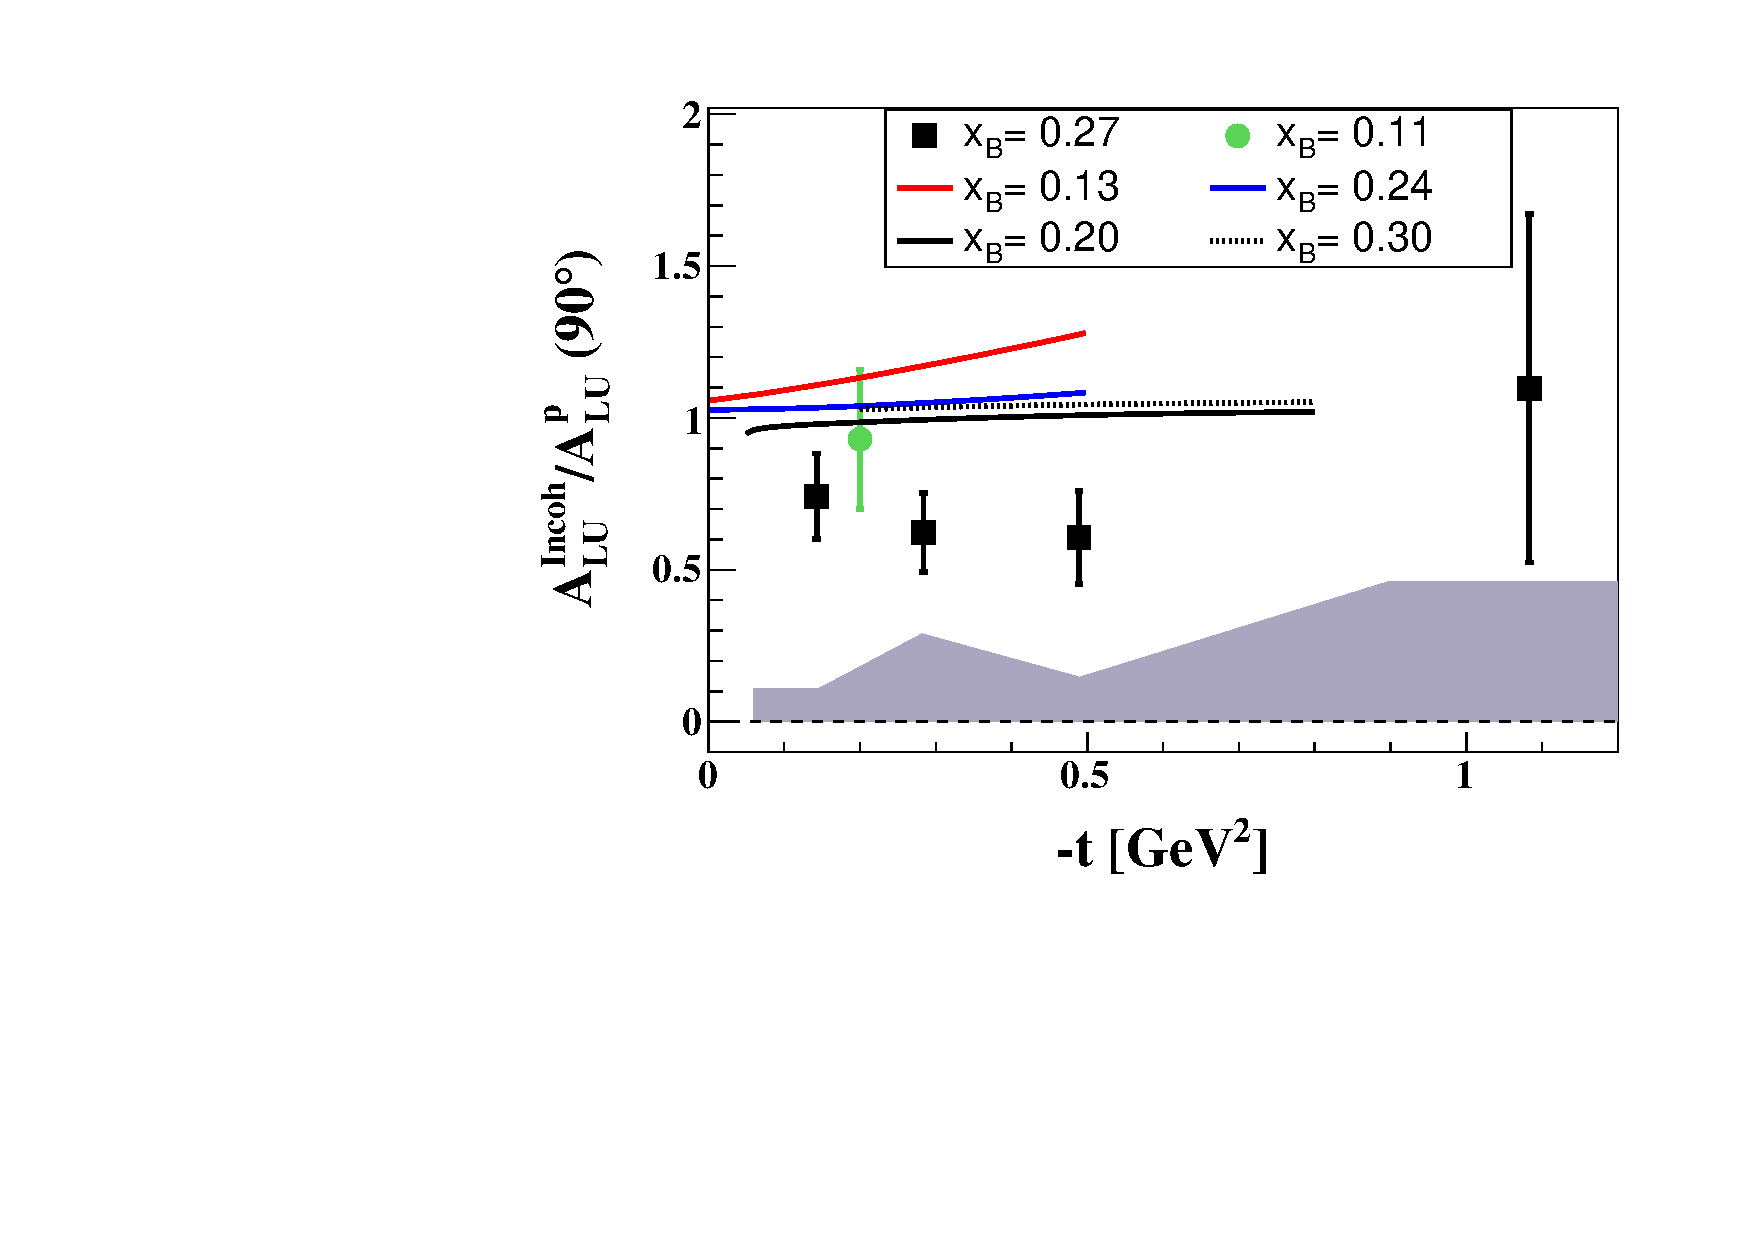
\includegraphics[width=6.9cm]{figs/ALU_ratioInc_t_shortscenrario.pdf}
\caption{ The $A_{LU}$ ratio of the bound to the free proton at 
   $\phi$~=~90$^{\circ}$, as a function of $Q^2$ (top), $x_B$ (middle), and $t$ 
   (bottom). The black squares are from this work, the green circles are the 
   HERMES inclusive measurement \cite{Airapetian}. The blue and red curves are 
   results of off-shell calculations \cite{simonetta_2}. The solid and dashed 
   black curves are from on-shell calculations \cite{Guzey:2008fe}.} 
   \label{fig:incoh_EMC_ratio_ALU_proton}
\end{figure}

The $A_{LU}$ ratios show a 20\%-40\% suppression in the bound protons compared 
to the free protons. These measurements disagree with the enhancement predicted 
by the on-shell calculations that use the medium modified GPDs as caluclated 
from the quark-meson coupling model \cite{Guzey:2008fe}. The off-shell 
calculations overshoot the data indicating a trend \cite{simonetta_2}. In
particular, the anti-shadowing region seems to be absent in terms of the 
$A_{LU}$ ratio, while it was predicted by the calculation. Within the given 
uncertainties, our measured ratios are compatible with the previous measured 
single point from HERMES \cite{Airapetian}.


These data, while limited in statistics, proved the experimental feasibility of 
measuring DVCS of bound-nucleons in addition to the EMC effect within the GPDs 
framework and led the way to the approval of a next generation nuclear 
measurements \cite{Armstrong:2017wfw}. The future measurements will be carried 
out using the new CLAS12 spectrometer and the upgraded CEBAF 12 GeV electron 
beam at an electron-nucleon luminosity of 10$^{35}$cm$^{-2}$s$^{-1}$. The wider 
accessible phase-space and the higher luminosity will enable us to study 
nuclear effects and their manifestations on GPDs including the effect of final 
state interactions.


%conclusion
In summary, we have presented the first exclusive beam-spin asymmetries 
associated with incoherent DVCS off $^4$He using an upgraded setup of CLAS 
spectrometer at Jefferson Lab. Our results were compared to some model 
calculations based on different assumptions of the nuclear medium effects at 
the partonic level and allowed us to draw some conclusions. The bound-proton 
beam-spin asymmetries indicate a suppression compared to the free proton 
results measured in similar phase-space. While the data are limited in 
statistics, they opened new insights for extensive future measurements.     

%Acknowledgments

The authors acknowledge the staff of the Accelerator and Physics Divisions at 
the Thomas Jefferson National Accelerator Facility who made this experiment 
possible. This work was supported in part by the Chilean Comisi\'on Nacional de 
Investigaci\'on Cient\'ifica y Tecnol\'ogica (CONICYT), the Italian Instituto 
Nazionale di Fisica Nucleare, the French Centre National de la Recherche 
Scientifique, the French Commissariat \`a l'Energie Atomique, the U.S.  
Department of Energy under Contract No. DE-AC02-06CH11357, the United Kingdom 
Science and Technology Facilities Council (STFC), the Scottish Universities 
Physics Alliance (SUPA), the National Research Foundation of Korea, and the 
Office of Research and Economic Development at Mississippi State University.  
M.~Hattawy also acknowledges the support of the Consulat G\'en\'eral de France 
\`a J\'erusalem.  The Southeastern Universities Research Association operates 
the Thomas Jefferson National Accelerator Facility for the United States 
Department of Energy under Contract No. DE-AC05-06OR23177.

\begin{thebibliography}{99}

%\cite{Hofstadter:1955ae}
\bibitem{Hofstadter:1955ae} R.~Hofstadter and R.~W.~McAllister,
%``Electron Scattering From the Proton,''
Phys.\ Rev.\  {\bf 98}, 217 (1955).
%doi:10.1103/PhysRev.98.217

%\cite{Perdrisat:2006hj}
\bibitem{Perdrisat:2006hj} C.~F.~Perdrisat, V.~Punjabi and M.~Vanderhaeghen,
%``Nucleon Electromagnetic Form Factors,''
Prog.\ Part.\ Nucl.\ Phys.\  {\bf 59}, 694 (2007)
%doi:10.1016/j.ppnp.2007.05.001
%[hep-ph/0612014].

%\cite{Dokshitzer:1977sg}
\bibitem{Dokshitzer:1977sg} Y.~L.~Dokshitzer,
%``Calculation of the Structure Functions for Deep Inelastic Scattering and e+ 
   %e- Annihilation by Perturbation Theory in Quantum Chromodynamics.,''
Sov.\ Phys.\ JETP {\bf 46}, 641 (1977)
[Zh.\ Eksp.\ Teor.\ Fiz.\  {\bf 73}, 1216 (1977)].

%\cite{pdg}
\bibitem{pdg} J.~Beringer {\it et al.} (Particle Data Group), Phys.\ Rev.\ D 
   {\bf 86}, 010001 (2012).

\bibitem{EMC_first}
   J.~J.~Aubert {\it et al.}, 
      %“The ratio of the nucleon structure functions F 2 n for iron and
      %deuterium,” 
      Phys.\ Lett.\, vol.\ B { \bf 123}, pp. 275–278 (1983).


\bibitem{EMC_CERN}
J. Ashman et al. (EMC Collaboration), 
      %Measurement of the ratios of deep inelastic muon-nucleus cross sections 
%on various nuclei compared to deuterium, 
      Phys.\ Lett.\ B\ {\bf 202}, 603 1988.

\bibitem{EMC_SLAC}
J. Gomez et al. (SLAC-E139), 
      %Measurement of the A dependence of deep-inelastic electron scattering, 
      Phys.\ Rev.\ D\ {\bf 49}, 4348 (1994).

\bibitem{EMC_HERMES}
A. Airapetian et al. (HERMES Collaboration), 
      %Nuclear effects on R = $\sigma_{L}/\sigma_{T}$ in deep-inelastic 
%scattering, 
      Phys.\ Lett.\ B\ {\bf 567}, 339 (2003).

\bibitem{EMC_JLab}
J. Seely et al., 
      %New Measurements of the European Muon Collaboration Effect in Very Light 
%Nuclei, 
      Phys.\ Rev.\ Lett.\ {\bf 103}, 202301 (2009).

\bibitem{EMC_John}
J. Arrington et al., 
%A detailed study of the nuclear dependence of the EMC effect and short-range 
%correlations, 
      Phys.\ Rev.\ C\ {\bf 86}, 065204 (2012).  

\bibitem{EMC_mdeium_1}
I. Clo\"et et al., 
%Isovector EMC effect explains the NuTeV anomaly, 
Phys.\ Rev.\ Lett.\ {\bf 102}, 252301 (2009).

\bibitem{EMC_medium_2}
I. Clo\"et et al., %Parity-violating DIS and the flavour dependence of the EMC 
%effect, 
Phys.\ Rev.\ Lett.\ {\bf 109}, 182301 (2012).


\bibitem{Mueller:1998fv} D. Mueller, D. Robaschik, B. Geyer, F.M. Dittes, and 
   J.  Horejsi,
Fortsch.\ Phys. {\bf 42}, 101 (1994).
  
\bibitem{Ji:1996ek} 
X.D. Ji,
Phys.\ Rev.\ Lett. {\bf 78}, 610 (1997).

\bibitem{Ji:1996nm} 
X.D. Ji,
Phys.\ Rev.\ D {\bf 55}, 7114 (1997).

\bibitem{Radyushkin:1996nd}
A.V. Radyushkin,
Phys.\ Lett.\  B {\bf 380}, 417 (1996).

\bibitem{Radyushkin:1997ki} 
A.V. Radyushkin,
Phys.\ Rev.\ D {\bf 56}, 5524 (1997).

\bibitem{Stepanyan:2001sm}
S.~Stepanyan {\it et al.} [CLAS Collaboration],
Phys.\ Rev.\ Lett. {\bf 87}, 182002 (2001).

\bibitem{Airapetian}
A. Airapetian {\it et al.} [HERMES Collaboration],
Phys.\ Rev.\ Lett. {\bf 87}, 182001 (2001);
JHEP {\bf 1207}, 032 (2012);
JHEP {\bf 1006}, 019 (2010);
JHEP {\bf 0806}, 066 (2008);
Phys.\ Lett.\ B {\bf 704}, 15 (2011);
Phys.\ Rev.\  D {\bf 75}, 011103 (2007);
JHEP {\bf 0911}, 083 (2009);
Phys.\ Rev.\ C {\bf 81}, 035202 (2010);
JHEP {\bf 1210}, 042 (2012).

\bibitem{Chekanov:2003ya}
S. Chekanov {\it et al.} [ZEUS Collaboration],
Phys.\ Lett.\  B {\bf 573}, 46 (2003).

\bibitem{Aktas:2005ty}
A. Aktas {\it et al.} [H1 Collaboration],
Eur.\ Phys.\ J.\ C {\bf 44}, 1 (2005).

\bibitem{Chen:2006na} 
S.~Chen {\it et al.} [CLAS Collaboration],
Phys.\ Rev.\ Lett.\ {\bf 97}, 072002 (2006).

\bibitem{Munoz Camacho:2006hx} 
C. Mu\~noz Camacho {\it et al.} [Jefferson Lab Hall A Collaboration],
Phys.\ Rev.\ Lett. {\bf 97}, 262002 (2006).

\bibitem{Girod:2007aa} 
F.X. Girod {\it et al.} [CLAS Collaboration],
Phys.\ Rev.\ Lett. {\bf 100}, 162002 (2008).

\bibitem{Mazouz:2007aa} 
   M.~Mazouz {\it et al.} [Jefferson Lab Hall A Collaboration],
   Phys.\ Rev.\ Lett.\  {\bf 99}, 242501 (2007)

\bibitem{Gavalian:2009} 
G. Gavalian {\it et al.} [CLAS Collaboration],
Phys.\ Rev.\ C {\bf 80}, 035206 (2009).

\bibitem{Seder:2015} 
E. Seder {\it et al.} [CLAS Collaboration],
Phys.\ Rev.\ Lett. {\bf 114}, 032001 (2015).

\bibitem{Pisano:2015} 
S.~Pisano {\it et al.} [CLAS Collaboration],
Phys.\ Rev.\ D {\bf 91}, 052014 (2015).

\bibitem{Jo:2015ema} H.~S.~Jo {\it et al.} [CLAS Collaboration],
  Phys.\ Rev.\ Lett.\  {\bf 115}, no. 21, 212003 (2015)

\bibitem{JSeely}
J. Seely {\it et al.}, Phys.\ Rev.\ Lett.\ {\bf 103}, 202301 (2009).


\bibitem{Dupre:2016mai} R.~Dupre, M.~Guidal and M.~Vanderhaeghen,
 %``Tomographic image of the proton,''
 Phys.\ Rev.\ D {\bf 95}, no. 1, 011501 (2017)

\bibitem{Hattawy:2017woc} 
   M.~Hattawy {\it et al.} [CLAS Collaboration],
   Phys.\ Rev.\ Lett.\  {\bf 119}, no. 20, 202004 (2017)


\bibitem{simonetta_2}
S.~Liuti and K.~Taneja, Phys.\ Rev.\ C {\bf 72}, 032201 (2005)

\bibitem{Guzey:2006xi} V.~Guzey and T.~Teckentrup, Phys.\ Rev.\ D {\bf 74}, 
   054027 (2006)

\bibitem{Guzey:2008fe} V.~Guzey, A.~W.~Thomas and K.~Tsushima,
  Phys.\ Lett.\ B {\bf 673}, 9 (2009)

\bibitem{Freund_Collins}
J.C.~Collins and A.~Freund, Phys.\ Rev.\ D {\bf 59}, 074009 (1999).

\bibitem{Ji_Osborne}
   X.-D.~Ji and J.~Osborne, Phys.\ Rev.\ D {\bf 58}, 094018 (1998).

\bibitem{Belitsky:2001ns}
A.~V.~Belitsky, D.~Mueller and A.~Kirchner,
Nucl.\ Phys.\ B {\bf 629}, 323 (2002)

\bibitem{Guidal:2013rya} M.~Guidal, H.~Moutarde, and M.~Vanderhaeghen,
Rep.\ Prog.\ Phys.\  {\bf 76}, 066202 (2013).


\bibitem{Hafidi:2008pr} K.~Hafidi {\it et al.},
   proposal PR-08-024 to JLab PAC33 (unpublished).

\bibitem{Mecking:2003zu} B.~A.~Mecking {\it et al.} [CLAS Collaboration],
   Nucl.\ Instrum.\ Meth.\ A {\bf 503}, 513 (2003).

\bibitem{Dupre:2017upj} R.~Dupr\'e {\it et al.},
  arXiv:1706.10160.

\bibitem{Hattawy:thesis}
M.~Hattawy, Ph.D. thesis, Universit{\'e} Paris Sud - Paris XI, France, 2015 
[Institution Report No. 2015PA112161].

%\cite{Armstrong:2017wfw}
\bibitem{Armstrong:2017wfw} W.~Armstrong {\it et al.},
     %``Partonic Structure of Light Nuclei,''
     arXiv:1708.00888 [nucl-ex].
       %%CITATION = ARXIV:1708.00888;%%
         %2 citations counted in INSPIRE as of 13 Feb 2018
     %\cite{Armstrong:2017zqr}
%\bibitem{Armstrong:2017zqr} W.~Armstrong {\it et al.},
       %``Tagged EMC Measurements on Light Nuclei,''
       arXiv:1708.00891 [nucl-ex].
         %%CITATION = ARXIV:1708.00891;%%
           %1 citations counted in INSPIRE as of 13 Feb 2018
       %\cite{Armstrong:2017zcm}
%    \bibitem{Armstrong:2017zcm} W.~R.~Armstrong {\it et al.},
         %``Spectator-Tagged Deeply Virtual Compton Scattering on Light 
       %Nuclei,''
         arXiv:1708.00835 [nucl-ex].
           %%CITATION = ARXIV:1708.00835;%%





\end{thebibliography}

\end{document}
